\documentclass[border=6pt]{standalone}
\usepackage{amsmath,amssymb}
\usepackage{tikz}
\usetikzlibrary{arrows.meta,calc,decorations.pathreplacing,patterns,shapes.geometric,positioning,shadings,decorations.pathmorphing}

\begin{document}
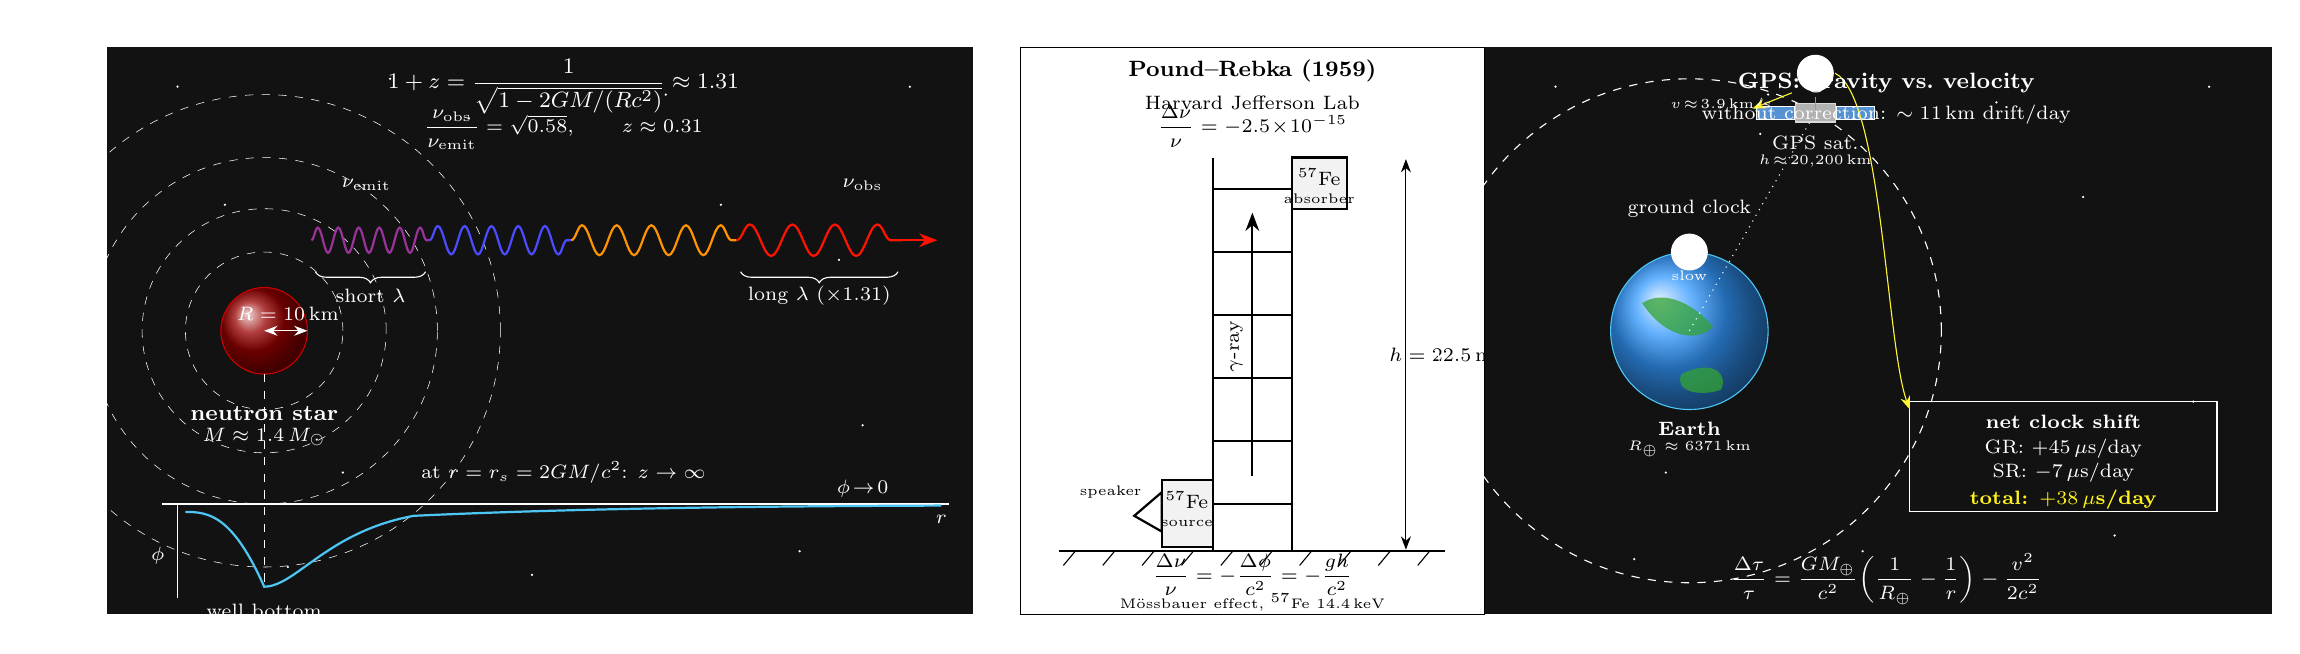
\begin{tikzpicture}[>=Stealth]

% ===========================================================
% LEFT PANEL: Neutron star gravitational well + climbing photon
% ===========================================================
\begin{scope}[local bounding box=left]

% Background sky
\fill[black!93] (-0.4,-3.6) rectangle (10.6,3.6);

% Faint stars
\foreach \x/\y in {0.5/3.1, 1.9/-3.0, 3.2/3.2, 5.0/-3.1, 6.7/3.0, 8.4/-2.8, 9.8/3.1, 2.6/-1.8, 7.4/1.6, 9.2/-1.2, 4.2/2.7, 8.9/0.9, 1.1/1.6}{
  \fill[white!80] (\x,\y) circle (0.45pt);
}

% Equipotential dashed rings around the neutron star (centered at (1.6,0))
\foreach \r in {1.0, 1.55, 2.2, 3.0}{
  \draw[white!40, dashed, very thin] (1.6,0) circle (\r);
}

% Neutron star (deep red sphere)
\shade[ball color=red!60!black] (1.6,0) circle (0.55);
\draw[red!80!black, thin] (1.6,0) circle (0.55);

% Radius label with a thin indicator
\draw[white!70, <->, thin] (1.6,0) -- (2.15,0);
\node[white, font=\scriptsize] at (1.9,0.22) {$R=10$\,km};

% Neutron star label
\node[white, font=\footnotesize\bfseries] at (1.6,-1.05) {neutron star};
\node[white, font=\scriptsize] at (1.6,-1.35) {$M\approx 1.4\,M_\odot$};

% --- Photon wavetrain: compact near surface, stretched far away ---
% Near-surface segment (tight wavelength, violet)
\draw[violet!80!white, thick, decorate, decoration={snake, amplitude=1.6mm, segment length=2.6mm}]
  (2.2,1.15) -- (3.7,1.15);
% Mid segment (blue)
\draw[blue!70!white, thick, decorate, decoration={snake, amplitude=1.8mm, segment length=3.4mm}]
  (3.7,1.15) -- (5.5,1.15);
% Orange segment (stretched)
\draw[orange!85!yellow, thick, decorate, decoration={snake, amplitude=1.9mm, segment length=4.4mm}]
  (5.5,1.15) -- (7.6,1.15);
% Red far segment (most stretched)
\draw[red!85!orange, thick, decorate, decoration={snake, amplitude=2.0mm, segment length=5.4mm}]
  (7.6,1.15) -- (9.7,1.15);

% Arrow at the end of photon path
\draw[red!85!orange, ->, thick] (9.7,1.15) -- (10.15,1.15);

% Photon label
\node[white, font=\scriptsize] at (2.9,1.85) {$\nu_{\text{emit}}$};
\node[white, font=\scriptsize] at (9.2,1.85) {$\nu_{\text{obs}}$};

% Brace beneath near-surface region labeling short lambda
\draw[white!75, decorate, decoration={brace, amplitude=4pt, mirror}]
  (2.25,0.75) -- (3.65,0.75);
\node[white, font=\scriptsize] at (2.95,0.45) {short $\lambda$};

% Brace beneath far region labeling long lambda (~1.31x)
\draw[white!75, decorate, decoration={brace, amplitude=4pt, mirror}]
  (7.65,0.75) -- (9.65,0.75);
\node[white, font=\scriptsize] at (8.65,0.45) {long $\lambda$ ($\times 1.31$)};

% Formula annotations (top)
\node[white, font=\footnotesize] at (5.4,3.1)
  {$1+z=\dfrac{1}{\sqrt{1-2GM/(Rc^{2})}}\approx 1.31$};
\node[white, font=\scriptsize] at (5.4,2.55)
  {$\dfrac{\nu_{\text{obs}}}{\nu_{\text{emit}}}=\sqrt{0.58},\qquad z\approx 0.31$};

% Gravitational potential well sketch at bottom
\draw[white!70, thin] (0.3,-2.2) -- (10.3,-2.2);
\node[white, font=\scriptsize] at (10.2,-2.4) {$r$};
\draw[white!70, thin] (0.5,-2.2) -- (0.5,-3.4);
\node[white, font=\scriptsize] at (0.25,-2.85) {$\phi$};
% Well curve
\draw[cyan!70, thick]
  (0.6,-2.3) .. controls (0.9,-2.3) and (1.2,-2.35) ..
  (1.6,-3.25) .. controls (2.0,-3.25) and (2.4,-2.55) ..
  (3.5,-2.35) .. controls (5.0,-2.28) and (7.0,-2.23) ..
  (10.2,-2.22);
% Well label
\node[white, font=\scriptsize] at (1.6,-3.55) {well bottom};
\node[white, font=\scriptsize] at (9.2,-2.0) {$\phi\!\to\!0$};

% Dashed drop line from star to well bottom
\draw[white!45, dashed, very thin] (1.6,-0.55) -- (1.6,-3.2);

% Horizon note
\node[white, font=\scriptsize] at (5.4,-1.8) {at $r=r_s=2GM/c^{2}$: $z\to\infty$};

\end{scope}

% ===========================================================
% MIDDLE PANEL: Pound-Rebka 22.5 m tower (1959)
% ===========================================================
\begin{scope}[xshift=11.5cm, local bounding box=mid]

% White background panel
\fill[white] (-0.3,-3.6) rectangle (5.6,3.6);
\draw[black, thin] (-0.3,-3.6) rectangle (5.6,3.6);

% Title
\node[black, font=\footnotesize\bfseries] at (2.65,3.3) {Pound--Rebka (1959)};
\node[black, font=\scriptsize] at (2.65,2.9) {Harvard Jefferson Lab};

% Ground line
\draw[black, thick] (0.2,-2.8) -- (5.1,-2.8);
\foreach \x in {0.4,0.9,1.4,1.9,2.4,2.9,3.4,3.9,4.4,4.9}{
  \draw[black, thin] (\x,-2.8) -- ++(-0.15,-0.18);
}

% Tower (two vertical lines)
\draw[black, thick] (2.15,-2.8) -- (2.15,2.2);
\draw[black, thick] (3.15,-2.8) -- (3.15,2.2);
% Horizontal braces
\foreach \y in {-2.2,-1.4,-0.6,0.2,1.0,1.8}{
  \draw[black, thin] (2.15,\y) -- (3.15,\y);
}

% Bottom box: gamma source + loudspeaker
\draw[black, thick, fill=black!5] (1.5,-2.75) rectangle (2.15,-1.9);
\node[black, font=\scriptsize] at (1.82,-2.15) {$^{57}$Fe};
\node[black, font=\tiny] at (1.82,-2.45) {source};
% Loudspeaker cone
\draw[black, thick] (1.15,-2.35) -- (1.5,-2.55) -- (1.5,-2.05) -- cycle;
\node[black, font=\tiny] at (0.85,-2.05) {speaker};

% Top box: absorber
\draw[black, thick, fill=black!5] (3.15,1.55) rectangle (3.85,2.2);
\node[black, font=\scriptsize] at (3.5,1.95) {$^{57}$Fe};
\node[black, font=\tiny] at (3.5,1.68) {absorber};

% Upward gamma photon arrow along tower center
\draw[black, ->, thick] (2.65,-1.85) -- (2.65,1.5);
\node[black, font=\scriptsize, rotate=90] at (2.45,-0.2) {$\gamma$-ray};

% Height label
\draw[black, <->, thin] (4.6,-2.78) -- (4.6,2.18);
\node[black, font=\scriptsize] at (5.05,-0.3) {$h=22.5$\,m};

% Delta nu / nu annotation
\node[black, font=\scriptsize] at (2.65,2.6)
  {$\dfrac{\Delta\nu}{\nu}=-2.5\!\times\!10^{-15}$};

% Weak-field formula at the base
\node[black, font=\scriptsize] at (2.65,-3.1)
  {$\dfrac{\Delta\nu}{\nu}=-\dfrac{\Delta\phi}{c^{2}}=-\dfrac{gh}{c^{2}}$};
\node[black, font=\tiny] at (2.65,-3.45) {M\"ossbauer effect, $^{57}$Fe 14.4\,keV};

\end{scope}

% ===========================================================
% RIGHT PANEL: Earth + GPS satellite clock shift
% ===========================================================
\begin{scope}[xshift=17.5cm, local bounding box=right]

% Sky background
\fill[black!93] (-0.4,-3.6) rectangle (9.6,3.6);

% faint stars
\foreach \x/\y in {0.5/3.1, 1.5/-2.9, 3.2/3.0, 4.4/-2.8, 6.1/2.9, 7.6/-2.6, 8.8/3.1, 1.9/-1.8, 7.2/1.7, 8.6/-0.9, 3.1/2.5}{
  \fill[white!80] (\x,\y) circle (0.45pt);
}

% Earth (blue sphere) at (2.2,0), radius 1.0 (symbolic 6371 km)
\shade[ball color=blue!50!cyan!80] (2.2,0) circle (1.0);
\draw[cyan!70!white, thin] (2.2,0) circle (1.0);
% Continent shapes
\fill[green!55!black!80, opacity=0.75]
  (1.6,0.35) .. controls (1.9,0.55) and (2.3,0.3) .. (2.5,0.05)
  .. controls (2.3,-0.15) and (1.9,-0.1) .. (1.6,0.35);
\fill[green!55!black!80, opacity=0.75]
  (2.1,-0.55) .. controls (2.5,-0.35) and (2.7,-0.55) ..
  (2.6,-0.75) .. controls (2.3,-0.85) and (2.0,-0.75) .. (2.1,-0.55);

% Ground clock at Earth surface (top of Earth)
\draw[white, thick, fill=white!10] (2.2,1.0) circle (0.22);
\draw[white, thin] (2.2,1.0) -- (2.2,1.18);
\draw[white, thin] (2.2,1.0) -- (2.32,0.97);
\node[white, font=\tiny] at (2.2,0.7) {slow};
\node[white, font=\scriptsize] at (2.2,1.55) {ground clock};

% Earth label
\node[white, font=\scriptsize\bfseries] at (2.2,-1.25) {Earth};
\node[white, font=\tiny] at (2.2,-1.5) {$R_\oplus\approx 6371$\,km};

% GPS orbit (symbolic scale)
\draw[white!55, dashed, thin] (2.2,0) circle (3.2);

% GPS satellite at top right of orbit (~60 deg up)
\coordinate (sat) at ($(2.2,0)+({3.2*cos(60)},{3.2*sin(60)})$);

% Satellite body (metallic gray)
\fill[gray!60] ($(sat)+(-0.25,-0.12)$) rectangle ($(sat)+(0.25,0.12)$);
\draw[gray!30, thin] ($(sat)+(-0.25,-0.12)$) rectangle ($(sat)+(0.25,0.12)$);
% Solar panels
\fill[cyan!55!blue!70] ($(sat)+(-0.75,-0.08)$) rectangle ($(sat)+(-0.27,0.08)$);
\fill[cyan!55!blue!70] ($(sat)+(0.27,-0.08)$) rectangle ($(sat)+(0.75,0.08)$);
\draw[white!40, very thin] ($(sat)+(-0.75,-0.08)$) rectangle ($(sat)+(-0.27,0.08)$);
\draw[white!40, very thin] ($(sat)+(0.27,-0.08)$) rectangle ($(sat)+(0.75,0.08)$);
% Antenna
\draw[gray!80, thin] (sat) -- ++(0,0.2);
% Satellite clock
\draw[white, thick, fill=white!10] ($(sat)+(0,0.5)$) circle (0.22);
\draw[white, thin] ($(sat)+(0,0.5)$) -- ++(0.1,0.12);
\draw[white, thin] ($(sat)+(0,0.5)$) -- ++(-0.1,-0.06);
\node[white, font=\tiny] at ($(sat)+(0,0.9)$) {fast};
\node[white, font=\scriptsize] at ($(sat)+(0,-0.38)$) {GPS sat.};
\node[white, font=\tiny] at ($(sat)+(0,-0.62)$) {$h\!\approx\!20{,}200$\,km};

% Orbital velocity arrow (tangential)
\draw[yellow!80, ->, thin] ($(sat)+(-0.3,0.25)$) -- ++(-0.5,-0.2);
\node[white, font=\tiny] at ($(sat)+(-1.2,0.1)$) {$v\!\approx\!3.9$\,km/s};

% Radial connecting line (for reference)
\draw[white!40, dotted, thin] (2.2,0) -- (sat);

% Net shift box
\draw[white!80, thin] (5.0,-2.3) rectangle (8.9,-0.9);
\node[white, font=\scriptsize\bfseries] at (6.95,-1.15) {net clock shift};
\node[white, font=\scriptsize] at (6.95,-1.50) {GR: $+45\,\mu$s/day};
\node[white, font=\scriptsize] at (6.95,-1.80) {SR: $-7\,\mu$s/day};
\node[yellow!90, font=\scriptsize\bfseries] at (6.95,-2.15) {total: $+38\,\mu$s/day};

% Arrow from satellite clock to the box
\draw[yellow!80, ->, thin] ($(sat)+(0.25,0.5)$) .. controls +(0.6,-0.3) and +(-0.3,0.8) .. (5.0,-1.0);

% Title
\node[white, font=\footnotesize\bfseries] at (4.7,3.15) {GPS: gravity vs.\ velocity};
\node[white, font=\scriptsize] at (4.7,2.75) {without correction: $\sim 11$\,km drift/day};

% Formula at bottom
\node[white, font=\scriptsize] at (4.7,-3.15)
  {$\dfrac{\Delta\tau}{\tau}=\dfrac{GM_\oplus}{c^{2}}\!\left(\dfrac{1}{R_\oplus}-\dfrac{1}{r}\right)-\dfrac{v^{2}}{2c^{2}}$};

\end{scope}

\end{tikzpicture}
\end{document}
